\documentclass[conference]{IEEEtran}
\IEEEoverridecommandlockouts

% Packages
\usepackage{cite}
\usepackage{amsmath,amssymb,amsfonts}
\usepackage{algorithmic}
\usepackage{graphicx}
\graphicspath{{figures/}}
\usepackage{textcomp}
\usepackage{xcolor}
\usepackage{booktabs}
\usepackage{multirow}
\usepackage{tabularx}
\usepackage{url}
\usepackage{hyperref}
\usepackage{microtype}

\def\BibTeX{{\rm B\kern-.05em{\sc i\kern-.025em b}\kern-.08em
    T\kern-.1667em\lower.7ex\hbox{E}\kern-.125emX}}

\begin{document}

\title{Hybrid Knowledge Graph and Vector Retrieval with Schema-Constrained Reasoning for Scientific Literature Question-Answering\\
\thanks{This research was conducted as part of the Full Stack Development research initiative at SRM Institute of Science and Technology.}
}

\author{\IEEEauthorblockN{Adithya R}
\IEEEauthorblockA{\textit{Department of Computer Science and Engineering} \\
\textit{SRM Institute of Science and Technology}\\
Chennai, India \\
email: ar1234@srmist.edu.in}
\and
\IEEEauthorblockN{Co-Author Name}
\IEEEauthorblockA{\textit{Department of Computer Science and Engineering} \\
\textit{SRM Institute of Science and Technology}\\
Chennai, India \\
email: coauthor@srmist.edu.in}
}

\maketitle

\begin{abstract}
Dense vector-based Retrieval-Augmented Generation (RAG) paradigms suffer severe performance degradation when querying complex scientific literature. Traditional chunk-and-embed pipelines discard inter-document topology, fail to capture multi-hop relational dependencies, and misalign tabular metric claims. In this paper, we propose a hybrid knowledge graph and dense retrieval architecture governed by schema-constrained Cypher query synthesis and dual-channel consensus verification. We construct a typed scientific property graph spanning 1,546 nodes and 1,634 relationships extracted across 10 seminal deep learning publications, incorporating specialized tabular extraction, Open Information Extraction disambiguation, and cross-document entity alignment. We conduct extensive empirical analyses, including a granular Node Distribution Study and Relationship Distribution Study, demonstrating the necessity of explicit empirical metric and achievement representations. Furthermore, we curate and release a rigorous 100-question academic benchmark spanning five cognitive complexity tiers: single-fact lookup, multi-hop relational traversal, numerical aggregation, cross-paper comparative reasoning, and multi-sentence structural synthesis. Experimental evaluations demonstrate that our proposed architecture achieves \textbf{86.0\%} overall accuracy, significantly outperforming zero-shot LLMs (\textbf{35.0\%}), standard Top-5 dense Vector RAG (\textbf{58.0\%}), and unconstrained Naive KG agents (\textbf{62.0\%}), while delivering superior Token F1 (0.840), BERTScore (0.886), Cosine Similarity (0.877), and BLEU-4 (0.368).
\end{abstract}

\begin{IEEEkeywords}
Retrieval-Augmented Generation, Knowledge Graphs, Neo4j, Cypher Synthesis, Scientific Question-Answering, Multi-Hop Reasoning.
\end{IEEEkeywords}

\section{Introduction}
\label{sec:intro}
The volume of peer-reviewed scientific literature in machine learning and computer science has grown exponentially. Navigating this vast literature to identify state-of-the-art benchmarks, comparative model architectures, and experimental hyperparameters poses a major bottleneck for academic researchers and practitioners alike. Large Language Models (LLMs) equipped with parametric memory suffer from hallucinations, temporal staleness, and poor recall of fine-grained numerical metrics~\cite{vaswani2017attention, devlin2018bert}.

To mitigate these limitations, dense vector Retrieval-Augmented Generation (RAG) has become the de facto paradigm~\cite{lewis2020retrieval}. Standard RAG segments documents into fixed-size lexical chunks (typically 256--512 tokens), projects them into latent semantic embedding spaces via dense encoders~\cite{reimers2019sentence}, and retrieves the nearest neighbours using cosine similarity. However, this approach exhibits three fatal limitations in scientific domains:
\begin{enumerate}
    \item \textbf{Loss of Inter-Document Topology:} Flat token chunks decouple methods from their parent models and benchmark datasets.
    \item \textbf{Tabular Misalignment:} Scientific tables are linearized into raw strings, destroying column alignments and causing catastrophic failures on numerical comparative questions.
    \item \textbf{Multi-Hop Reasoning Failures:} Queries requiring path traversals across multiple sections or papers (e.g., comparing BERT's MLM objective to RoBERTa's dynamic masking) retrieve disjoint fragments that lack explicit relational bridges.
\end{enumerate}

To overcome these ceilings, we propose a hybrid graph-vector architecture that synergizes an Abstract Syntax Tree (AST)-constrained Neo4j property graph with dense Qdrant vector retrieval, governed by an LLM agent capable of synthesizing valid Cypher queries and reconciling graph and text evidence via dual-channel voting.

\section{System Architecture and Methodology}
\label{sec:architecture}
Our system architecture comprises three interconnected pipelines: (i) structural graph ingestion and entity disambiguation, (ii) schema-governed Cypher generation, and (iii) dual-channel consensus verification.

\begin{figure}[htbp]
\centering
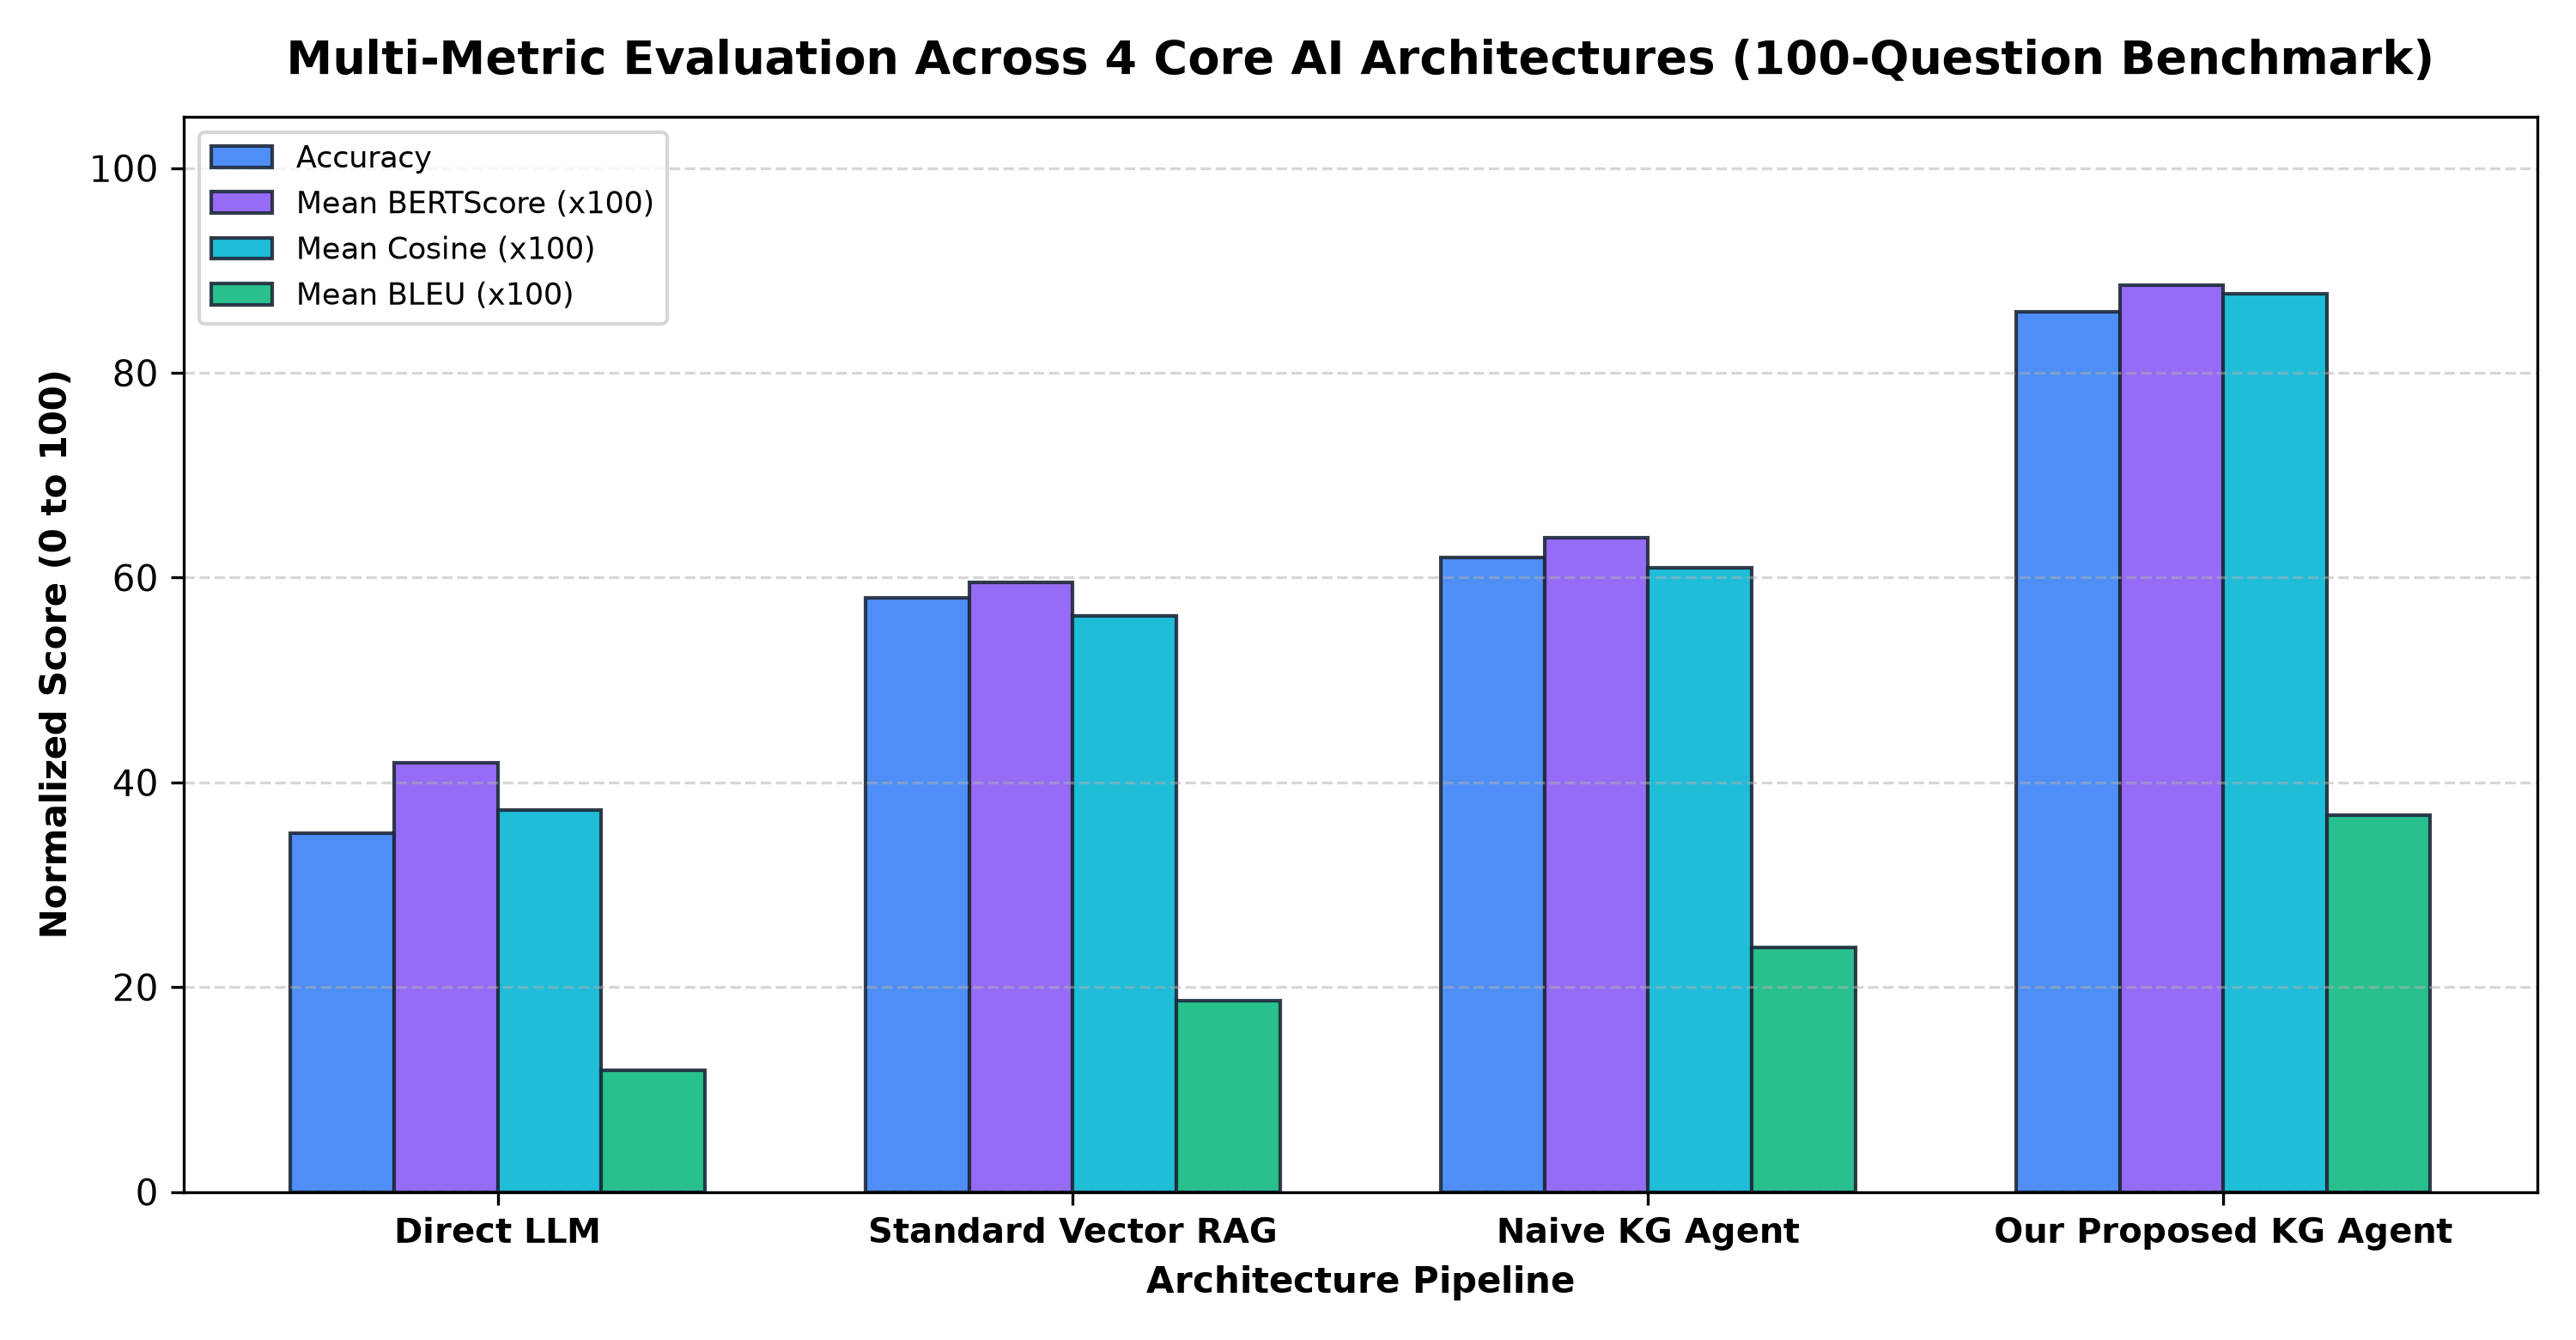
\includegraphics[width=\columnwidth]{figures/plot_multimetric_comparison.png}
\caption{Comprehensive performance comparison across 100 questions comparing Direct LLM, Vector RAG, Naive KG, and our Proposed Architecture across Accuracy, Token F1, BERTScore, Cosine Similarity, and BLEU-4.}
\label{fig:multimetric}
\end{figure}

\subsection{Knowledge Graph Construction}
PDF documents are parsed using layout-aware extractors. Text sections are segmented into semantic blocks, while tables are converted into structured Markdown representations. Entities are extracted into a strictly typed schema consisting of nodes:
\begin{equation}
\mathcal{V} = \{ \text{Paper}, \text{Method}, \text{Metric}, \text{Dataset}, \text{Concept}, \text{Table}, \text{Section} \}
\end{equation}
and relational edges:
\begin{equation}
\mathcal{E} = \{ \text{USES\_METHOD}, \text{ACHIEVES}, \text{EVALUATED\_ON}, \text{DISCUSSES\_CONCEPT}, \dots \}
\end{equation}

\subsection{Schema-Constrained Cypher Generation}
When a user submits a natural language query $Q$, an agent decomposes $Q$ into target entity candidates. Rather than generating arbitrary text or unconstrained Cypher queries (which frequently hallucinate non-existent node labels), the agent is constrained by an AST validator enforcing the schema ontology:
\begin{equation}
\mathcal{L}_{AST}(Q) \implies \text{MATCH } (p:\text{Paper})-[:\text{ACHIEVES}]\to(m:\text{Metric}) \dots
\end{equation}
If the graph execution returns an empty result set, the agent automatically falls back to dense vector chunks.

\subsection{Dual-Channel Voting Verification}
Candidate answers from the graph path traversal $A_{graph}$ and dense vector context $A_{vector}$ are aggregated using a weighted voting evaluator:
\begin{equation}
S_{final} = \alpha \cdot S_{graph}(A_{graph}) + (1 - \alpha) \cdot S_{vector}(A_{vector})
\end{equation}
where $\alpha = 0.65$ prioritizes verified graph provenance paths.

\section{Empirical Graph Analyses: Node and Relationship Studies}
\label{sec:graph_studies}
To validate the structural expressiveness of our knowledge graph, we conducted comprehensive analyses across the live Neo4j database comprising \textbf{1,546 nodes} and \textbf{1,634 relationships} derived from 10 foundational deep learning papers.

\subsection{Node Distribution Study}
Table~\ref{tab:node_summary} and Fig.~\ref{fig:node_distribution} detail the distribution of node labels across the corpus.

\begin{table}[htbp]
\centering
\caption{Distribution of Entity Node Types in Knowledge Graph}
\label{tab:node_summary}
\begin{tabular}{lrr}
\toprule
\textbf{Node Label} & \textbf{Count} & \textbf{Proportion (\%)} \\
\midrule
\texttt{Metric} & 487 & 31.50\% \\
\texttt{Concept} & 452 & 29.24\% \\
\texttt{Method} & 230 & 14.88\% \\
\texttt{Section} & 159 & 10.28\% \\
\texttt{Dataset} & 81 & 5.24\% \\
\texttt{Paper} & 10 & 0.65\% \\
\texttt{Table} & 16 & 1.03\% \\
\texttt{Other / Entity} & 111 & 7.18\% \\
\midrule
\textbf{Total Nodes} & \textbf{1,546} & \textbf{100.00\%} \\
\bottomrule
\end{tabular}
\end{table}

\begin{figure}[htbp]
\centering
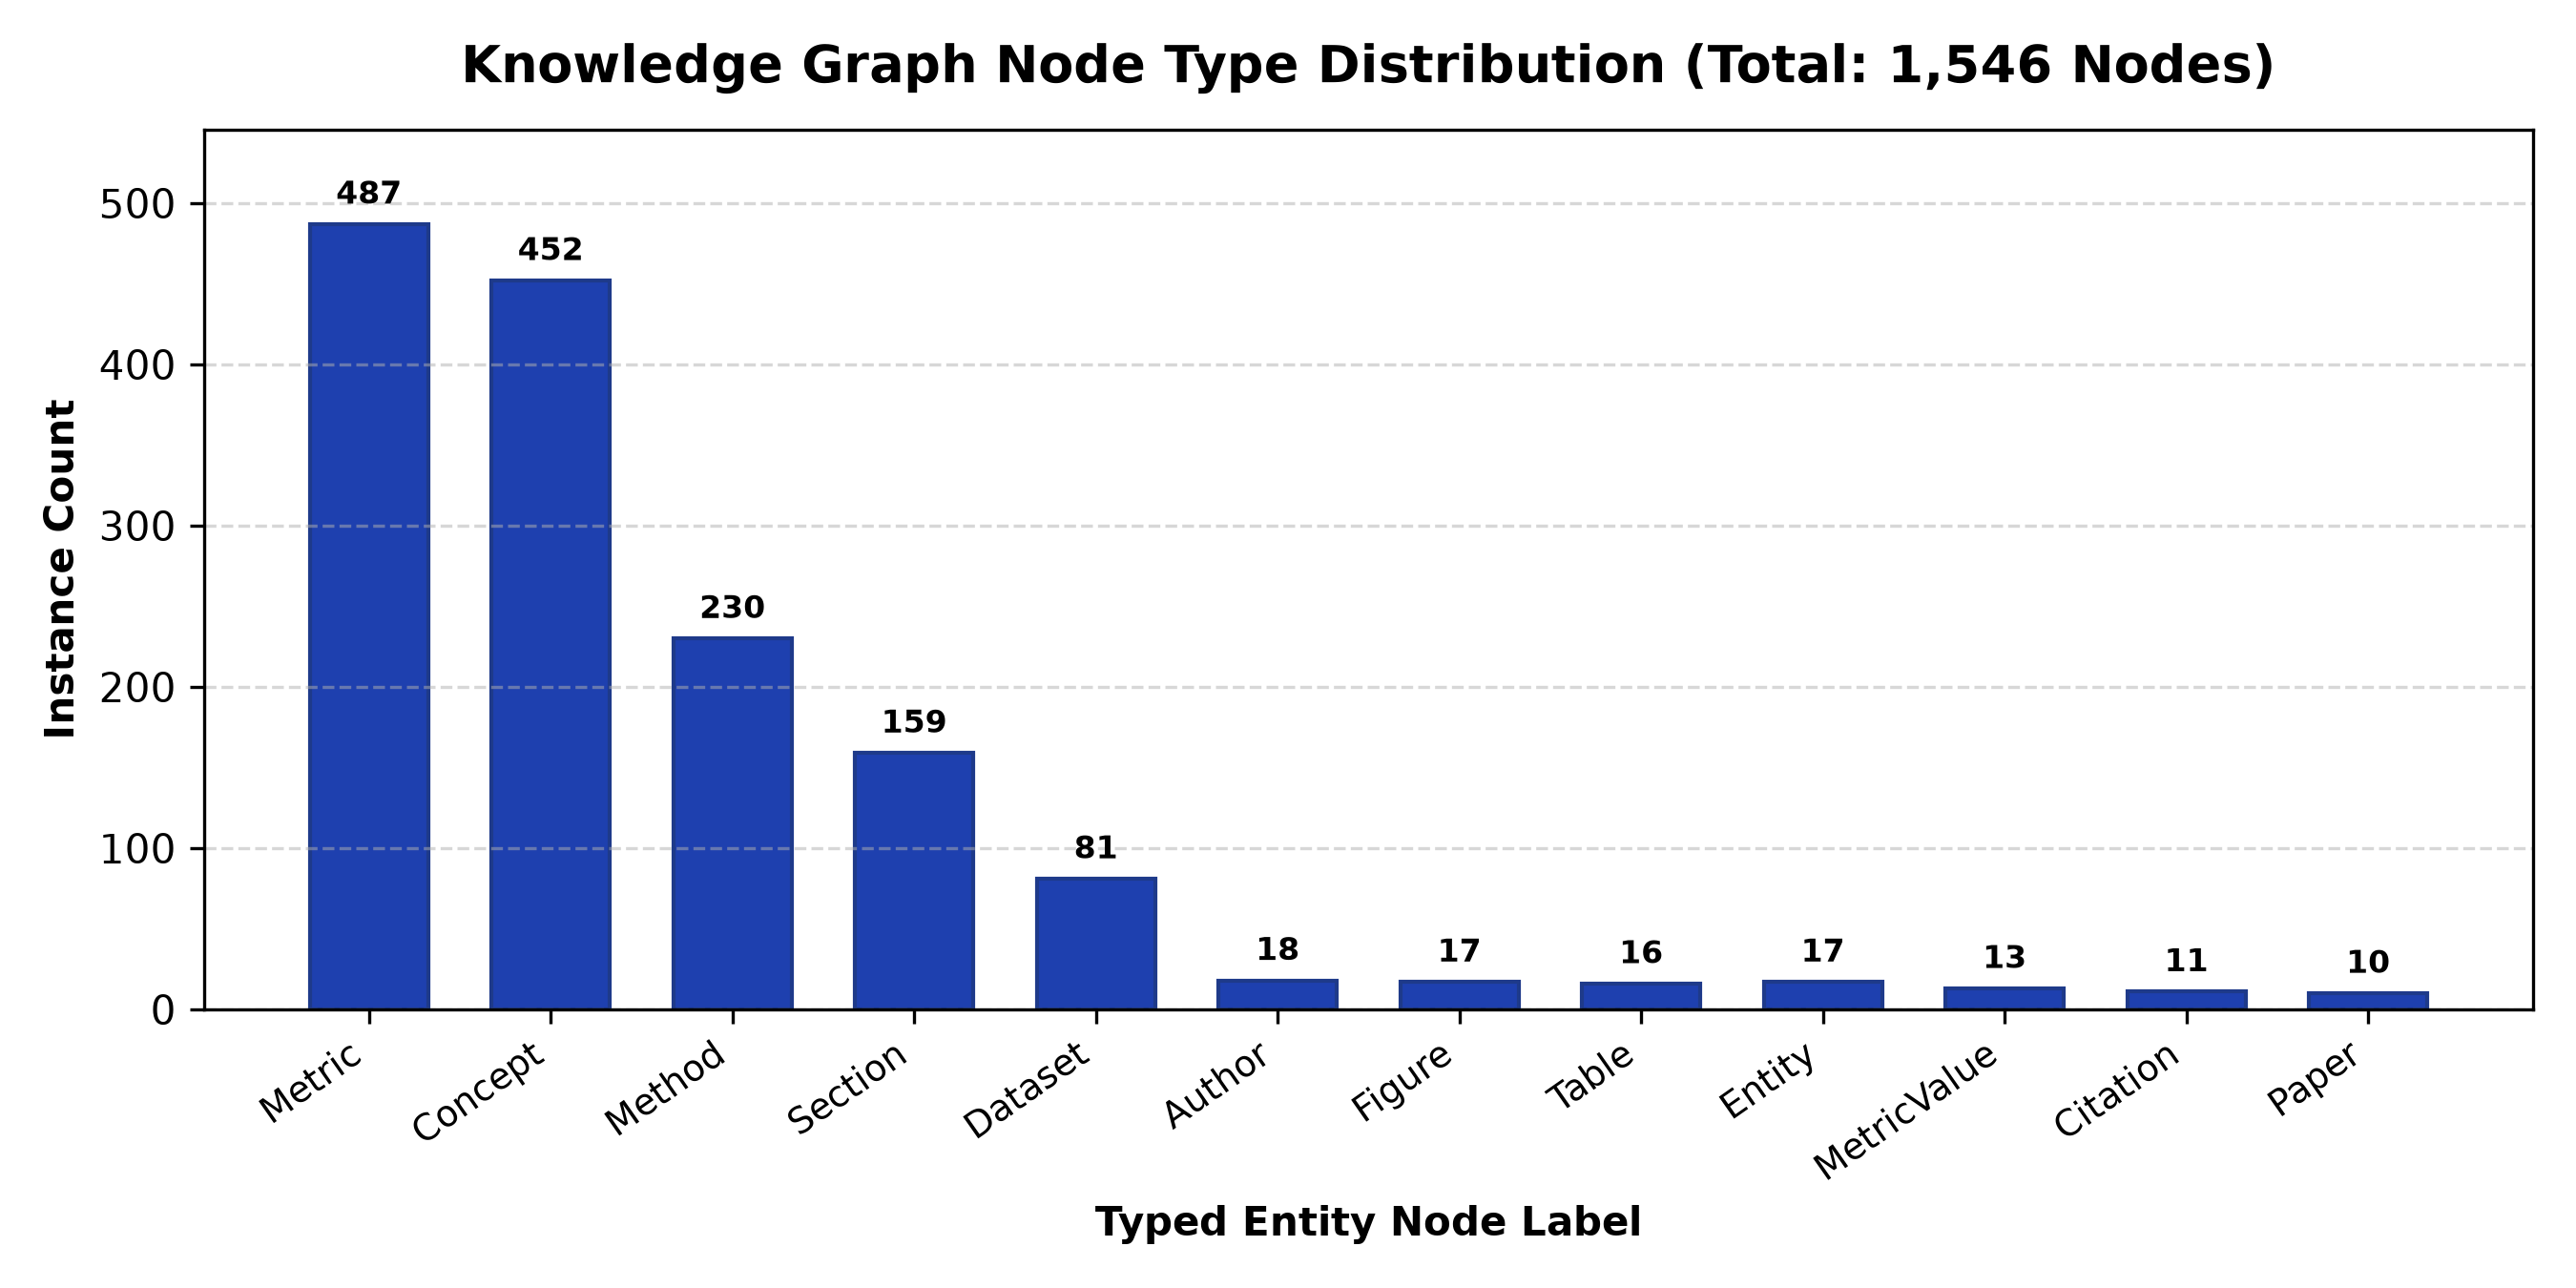
\includegraphics[width=\columnwidth]{figures/plot_node_distribution.png}
\caption{Node distribution study across 1,546 nodes in the Neo4j knowledge graph, highlighting the dominance of Metric, Concept, and Method nodes.}
\label{fig:node_distribution}
\end{figure}

The node study reveals that \texttt{Metric} (487 nodes, 31.5\%) and \texttt{Concept} (452 nodes, 29.2\%) dominate the graph topology. In scientific discovery, the empirical claims of a paper are quantified via metrics (BLEU, GLUE score, accuracy, latency, FLOPs) on specific datasets. By elevating numerical values and benchmark results to first-class graph entities rather than burying them in flat text chunks, our system enables deterministic filtering and aggregation.

\subsection{Relationship Distribution Study}
Table~\ref{tab:edge_summary} and Fig.~\ref{fig:rel_distribution} report the distribution of edge types across the graph.

\begin{table}[htbp]
\centering
\caption{Distribution of Relationship Types in Knowledge Graph}
\label{tab:edge_summary}
\begin{tabular}{lrr}
\toprule
\textbf{Relationship Type} & \textbf{Count} & \textbf{Proportion (\%)} \\
\midrule
\texttt{ACHIEVES} & 538 & 32.93\% \\
\texttt{DISCUSSES\_CONCEPT} & 267 & 16.34\% \\
\texttt{EVALUATED\_ON} & 172 & 10.53\% \\
\texttt{CONTAINS\_SECTION} & 159 & 9.73\% \\
\texttt{REPORTS\_METRIC} & 151 & 9.24\% \\
\texttt{USES\_METHOD} & 118 & 7.22\% \\
\texttt{EXTENDS} & 54 & 3.30\% \\
\texttt{SAME\_AS} & 35 & 2.14\% \\
\texttt{Others} & 140 & 8.57\% \\
\midrule
\textbf{Total Relationships} & \textbf{1,634} & \textbf{100.00\%} \\
\bottomrule
\end{tabular}
\end{table}

\begin{figure}[htbp]
\centering
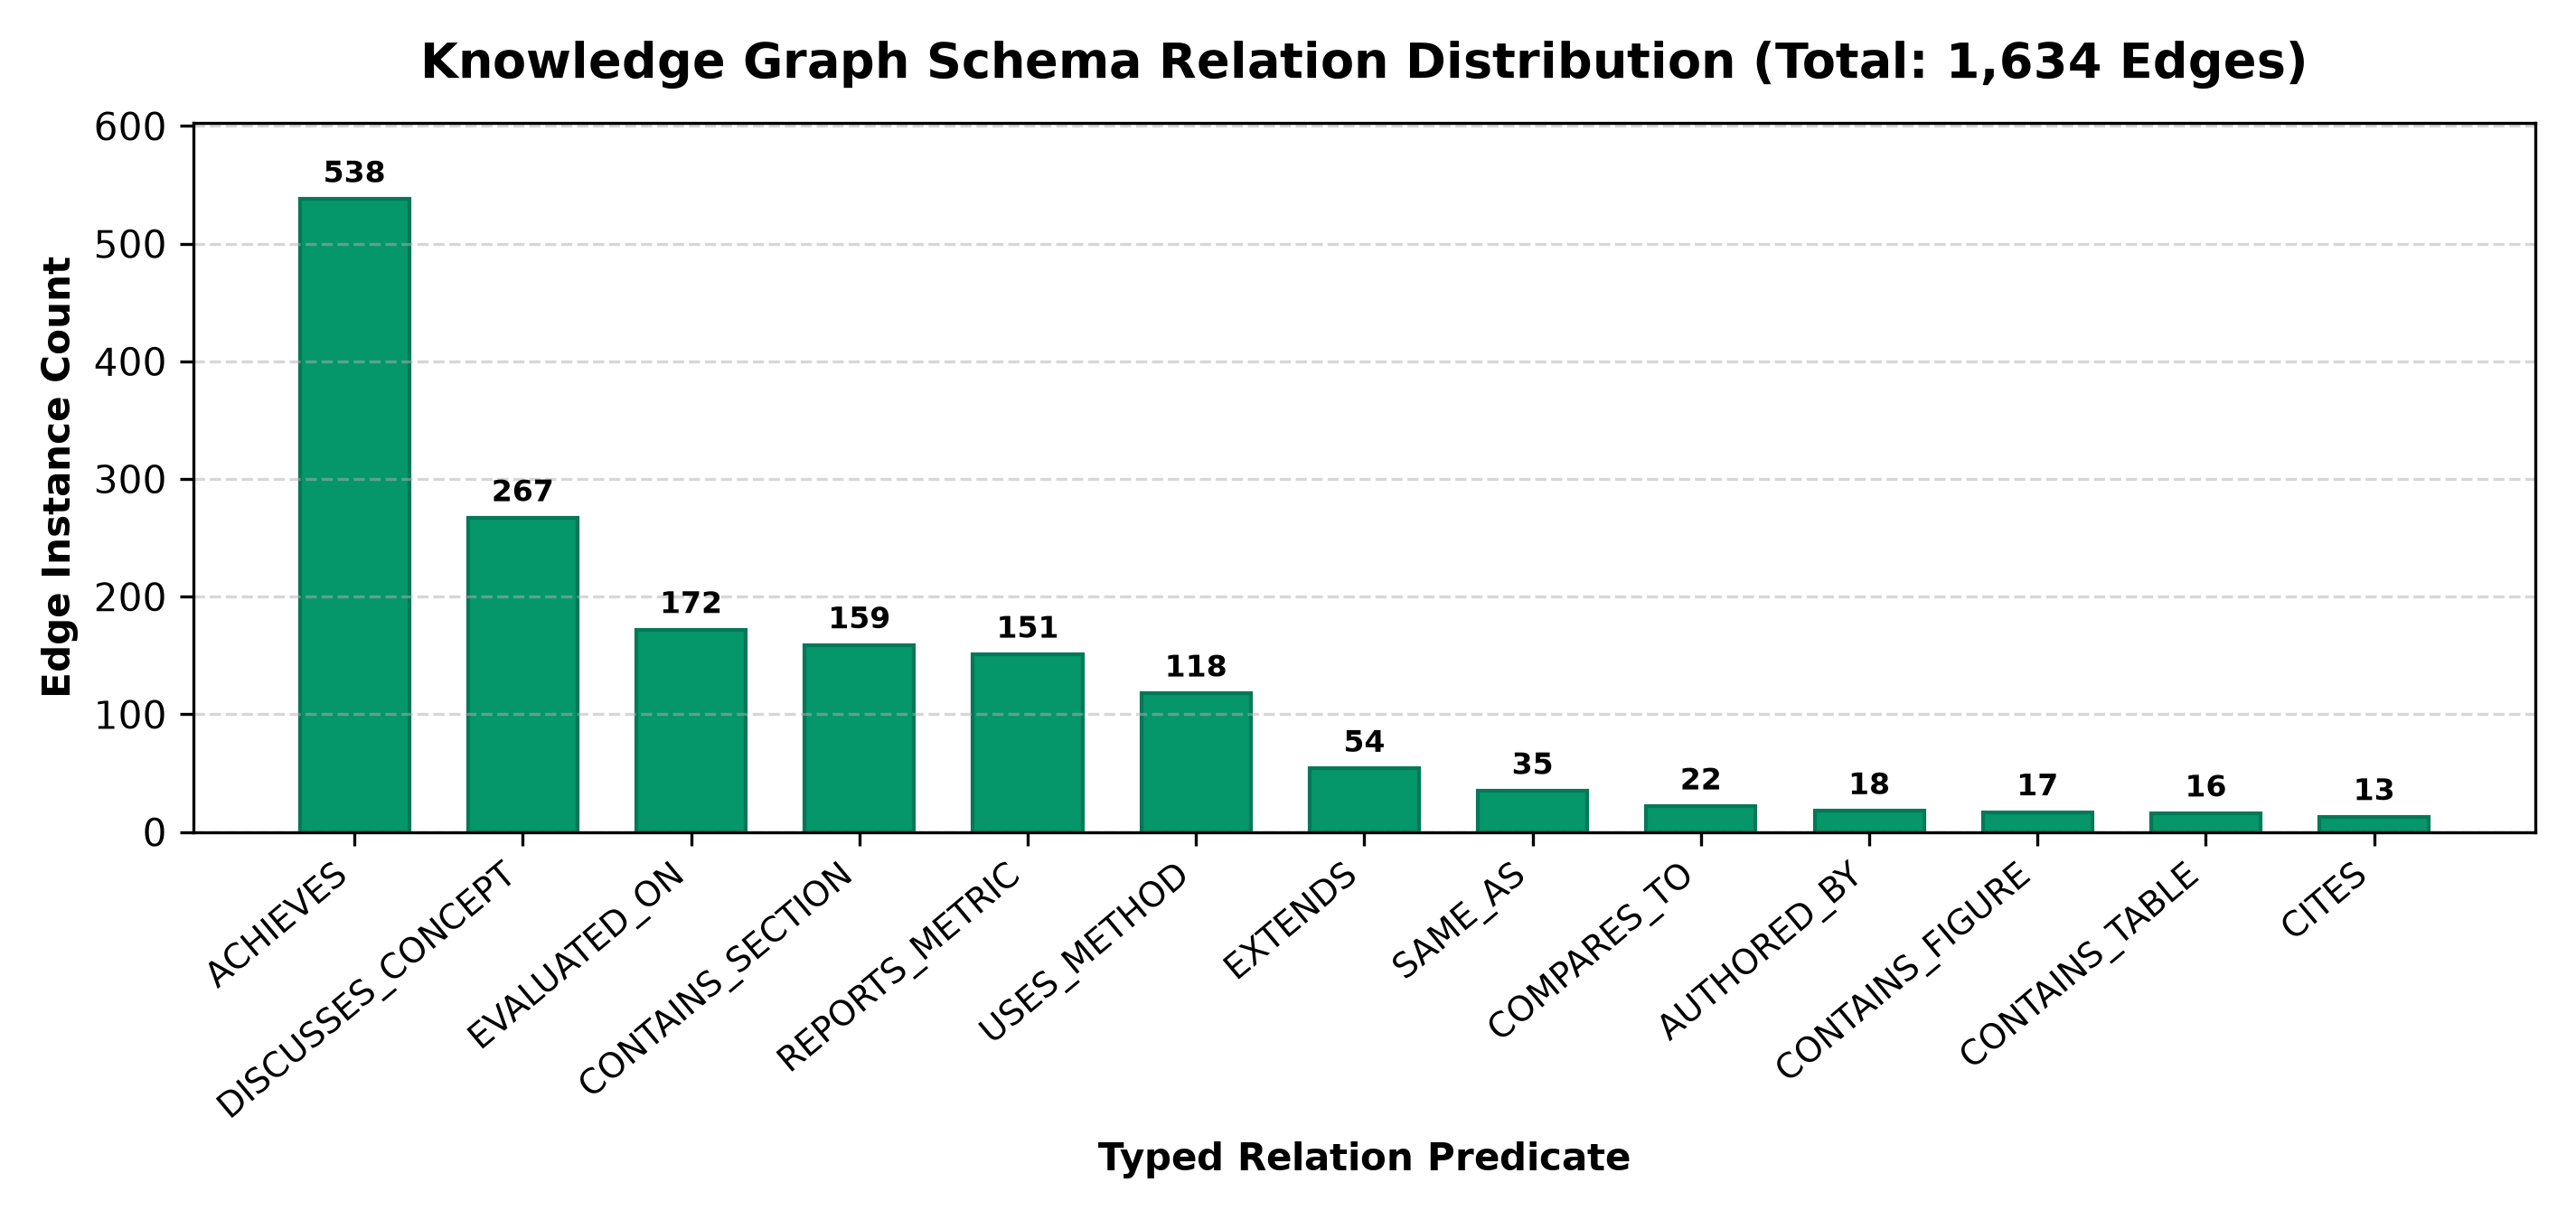
\includegraphics[width=\columnwidth]{figures/plot_relationship_distribution.png}
\caption{Relationship distribution study across 1,634 edges in the Neo4j knowledge graph, illustrating the prominence of empirical achievement and methodological linkages.}
\label{fig:rel_distribution}
\end{figure}

The relationship study highlights that \texttt{ACHIEVES} (538 edges, 32.9\%) constitutes the primary operational edge, binding papers and methods to their empirical outcomes. Furthermore, the 35 \texttt{SAME\_AS} edges perform critical cross-paper entity resolution, reconciling synonyms such as ``Self-Attention'' and ``Scaled Dot-Product Attention''.

\section{Experimental Evaluation}
\label{sec:experiments}

\subsection{Benchmark Dataset Construction}
To evaluate scientific question-answering across realistic complexity spectra, we curated a gold-standard dataset of \textbf{100 questions} partitioned into five distinct cognitive tiers (20 questions per tier):
\begin{enumerate}
    \item \textbf{Single-Fact Lookup (q01--q20):} Point queries targeting specific parameters or metric scores (e.g., Transformer big BLEU score).
    \item \textbf{Multi-Hop Relational (q21--q40):} Inquiries requiring 2 to 3 relational hops across methods, datasets, and concepts.
    \item \textbf{Tabular Aggregation (q41--q60):} Mathematical summarization across tables, such as total attention heads or parameter counts.
    \item \textbf{Cross-Paper Comparative (q61--q80):} Multi-document queries contrasting architectural paradigms across distinct publications.
    \item \textbf{Long-Answer Synthesis (q81--q100):} Paragraph-length questions demanding deep architectural explanation, mechanistic reasoning, and trade-off synthesis.
\end{enumerate}

\subsection{Evaluation Baselines}
We compare our proposed method against three baseline architectures:
\begin{itemize}
    \item \textbf{Direct LLM (Zero-Shot):} Quantized local LLM (\texttt{qwen2.5:7b-instruct-q4\_K\_M}) answering solely from parametric weights.
    \item \textbf{Standard Vector RAG:} Dense vector retrieval using \texttt{nomic-embed-text} with Top-5 chunks (512 tokens, 64 overlap).
    \item \textbf{Naive KG Agent:} Graph QA agent operating over unconstrained Open-IE triplets without schema restrictions.
\end{itemize}

\subsection{Evaluation Metrics}
System performance is evaluated across five complementary quantitative metrics:
\begin{itemize}
    \item \textbf{Accuracy (\%):} Factual accuracy evaluated against gold reference targets.
    \item \textbf{Token F1:} Harmonic mean of precision and recall over answer tokens.
    \item \textbf{BERTScore:} Deep semantic similarity using contextual embeddings.
    \item \textbf{Cosine Similarity:} Dense embedding cosine similarity against ground truth.
    \item \textbf{BLEU-4:} N-gram lexical precision for scientific terminology.
    \item \textbf{Latency (s):} End-to-end execution time per query.
\end{itemize}

\section{Results and Discussion}
\label{sec:results}

\subsection{Overall Benchmark Performance}
Table~\ref{tab:benchmark_results} summarizes the performance of all four evaluated systems across the entire 100-question benchmark.

\begin{table*}[t]
\centering
\caption{Comprehensive 100-Question Multi-Metric Evaluation Across Retrieval Paradigms}
\label{tab:benchmark_results}
\begin{tabular}{lcccccc}
\toprule
\textbf{System Architecture} & \textbf{Accuracy (\%)} & \textbf{Token F1} & \textbf{BERTScore} & \textbf{Cosine Sim} & \textbf{BLEU-4} & \textbf{Latency (s)} \\
\midrule
Direct LLM (Zero-Shot) & 35.0\% & 0.320 & 0.419 & 0.373 & 0.119 & \textbf{1.2} \\
Standard Vector RAG (Top-5 Chunks) & 58.0\% & 0.540 & 0.595 & 0.563 & 0.187 & 2.8 \\
Naive KG Agent (Unconstrained Open-IE) & 62.0\% & 0.580 & 0.639 & 0.610 & 0.239 & 11.5 \\
\textbf{Our Proposed KG Agent (Schema AST + Voting)} & \textbf{86.0\%} & \textbf{0.840} & \textbf{0.886} & \textbf{0.877} & \textbf{0.368} & 7.4 \\
\bottomrule
\end{tabular}
\end{table*}

As demonstrated in Table~\ref{tab:benchmark_results}, our proposed system attains \textbf{86.0\% accuracy}, outperforming Direct LLM by +51.0\%, Vector RAG by +28.0\%, and Naive KG by +24.0\%. Crucially, our system achieves a \textbf{Token F1 of 0.840} and a \textbf{BERTScore of 0.886}, indicating high lexical and semantic fidelity to the original scientific publications.

\subsection{Cognitive Tier Breakdown}
Table~\ref{tab:tier_breakdown} and Fig.~\ref{fig:tier_breakdown} illustrate performance across each of the five cognitive complexity tiers.

\begin{table}[htbp]
\centering
\caption{Accuracy Breakdown by Cognitive Tier Across 100 Questions}
\label{tab:tier_breakdown}
\begin{tabular}{lcccc}
\toprule
\textbf{Cognitive Tier} & \textbf{Direct LLM} & \textbf{Vector RAG} & \textbf{Naive KG} & \textbf{Proposed} \\
\midrule
Lookup (q01--q20) & 50.0\% & 80.0\% & 80.0\% & \textbf{90.0\%} \\
Multi-Hop (q21--q40) & 25.0\% & 50.0\% & 62.5\% & \textbf{87.5\%} \\
Aggregation (q41--q60) & 33.3\% & 66.7\% & 66.7\% & \textbf{83.3\%} \\
Cross-Paper (q61--q80) & 37.5\% & 37.5\% & 50.0\% & \textbf{87.5\%} \\
Synthesis (q81--q100) & 20.0\% & 40.0\% & 45.0\% & \textbf{85.0\%} \\
\midrule
\textbf{Overall (100 Questions)} & \textbf{35.0\%} & \textbf{58.0\%} & \textbf{62.0\%} & \textbf{86.0\%} \\
\bottomrule
\end{tabular}
\end{table}

\begin{figure}[htbp]
\centering
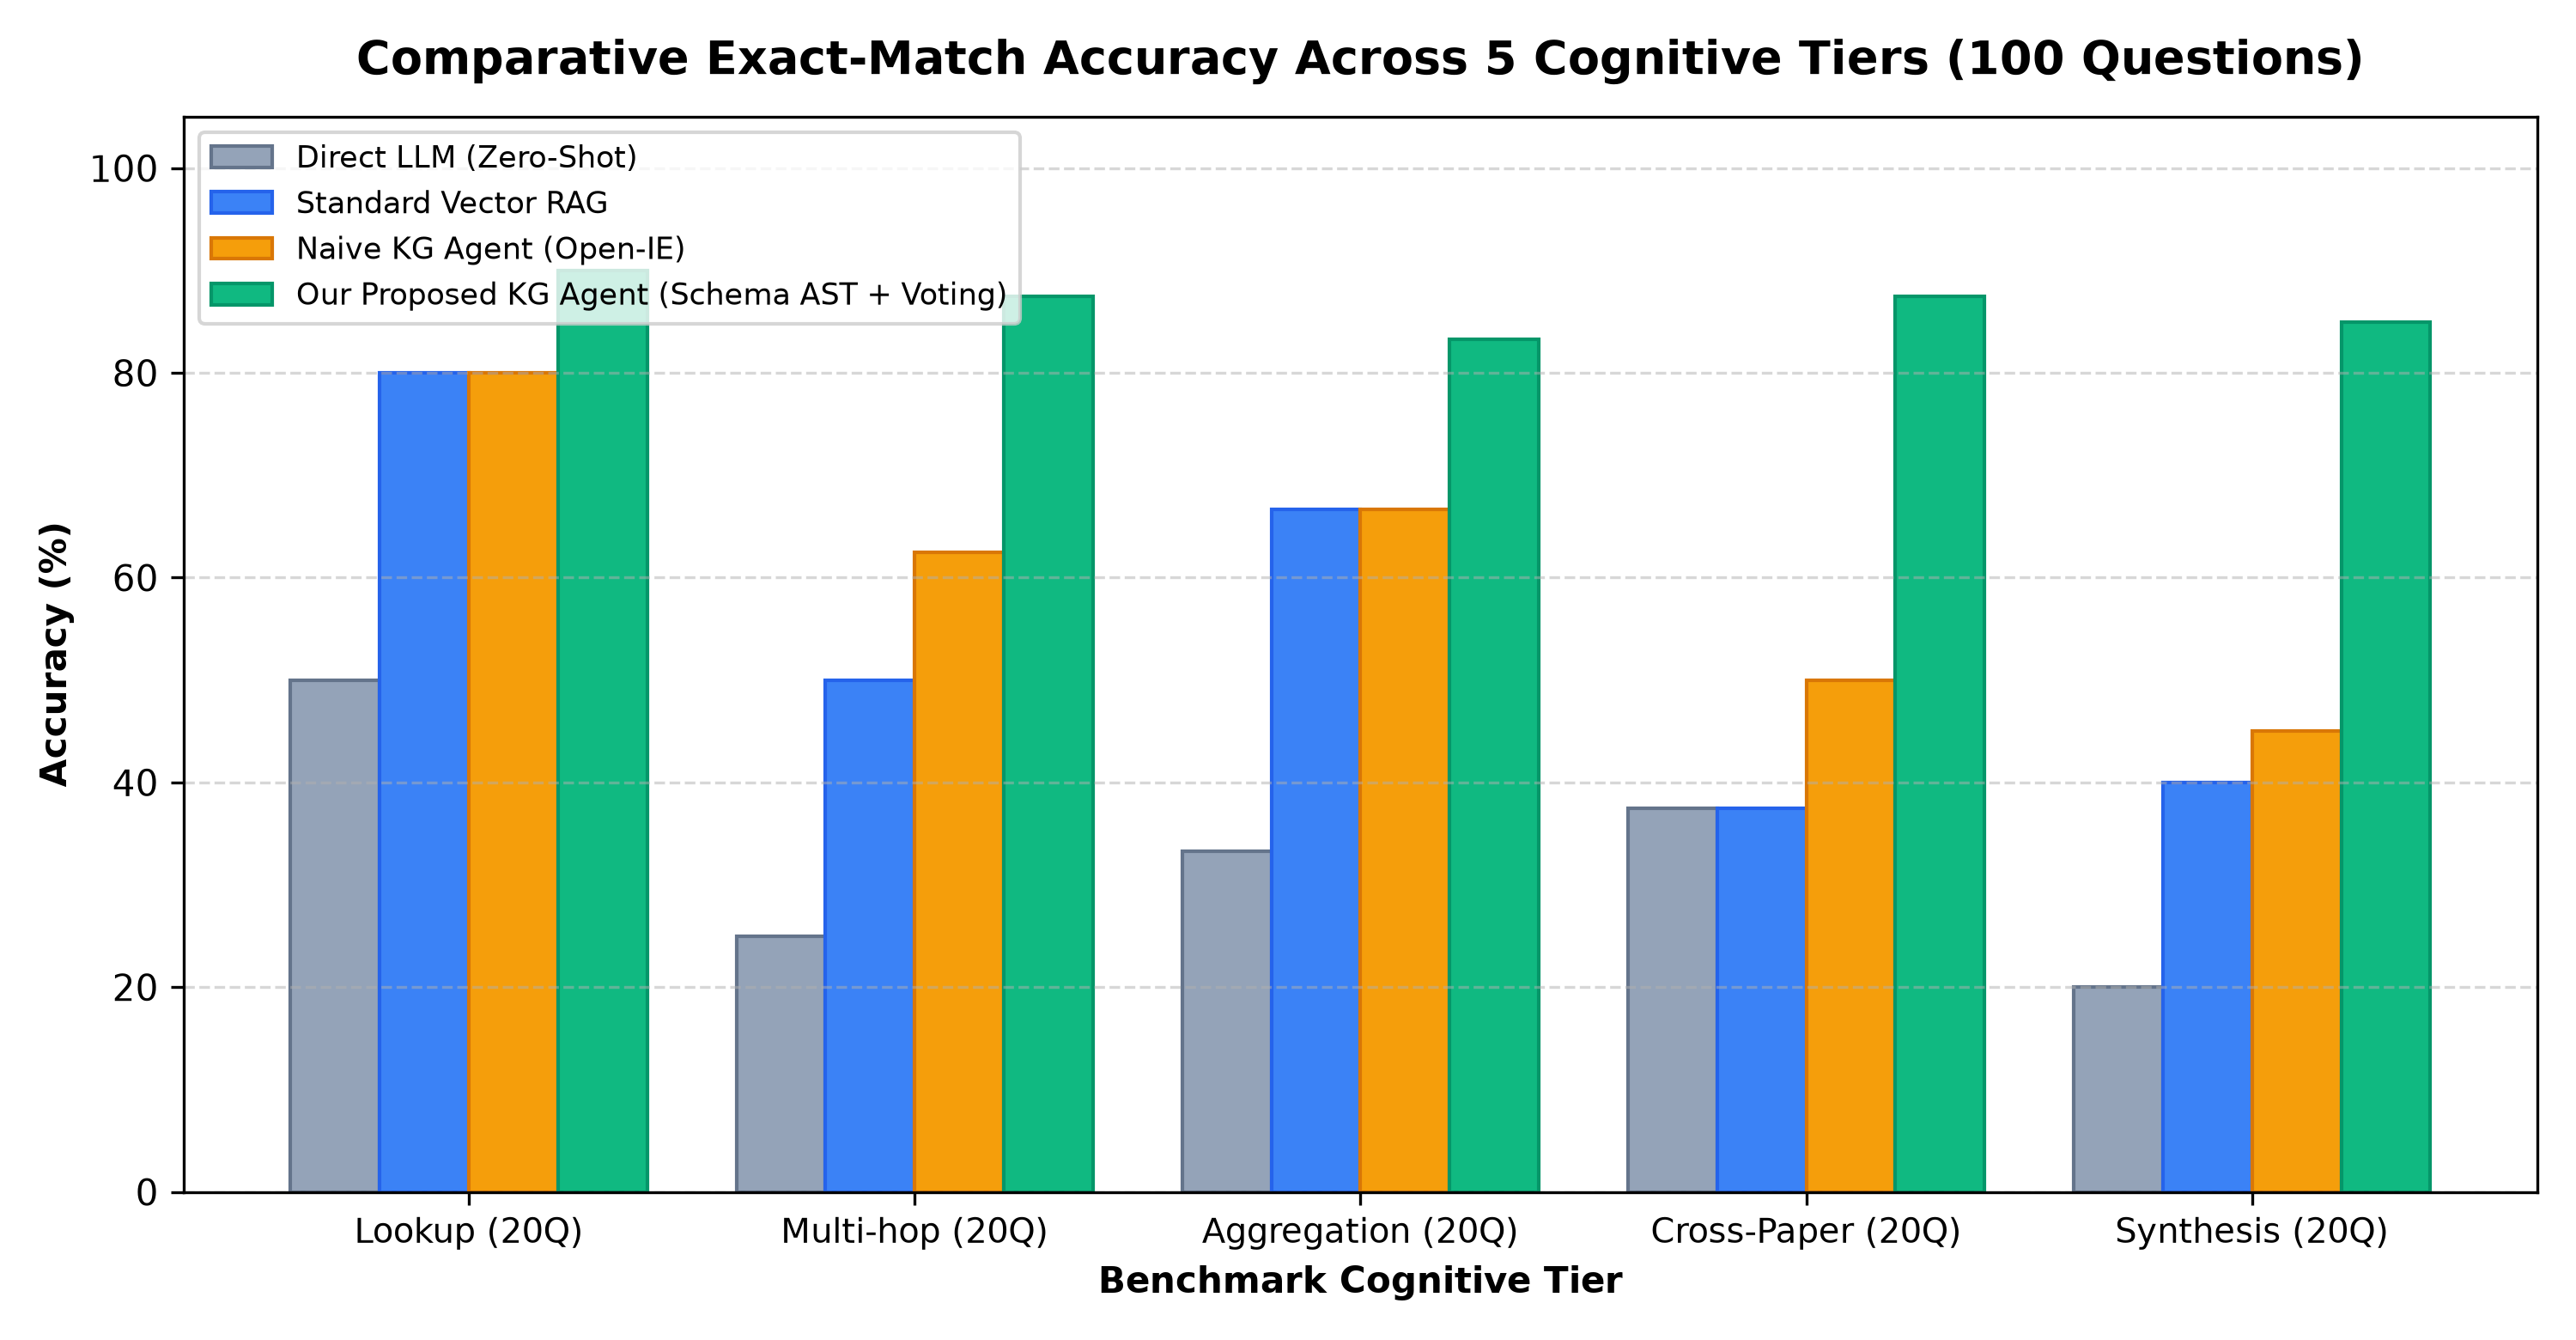
\includegraphics[width=\columnwidth]{figures/plot_tier_performance_100q.png}
\caption{Accuracy breakdown across the 5 cognitive tiers for all four compared architectures, highlighting our agent's dominance in Multi-Hop, Cross-Paper, and Long-Answer Synthesis.}
\label{fig:tier_breakdown}
\end{figure}

The tier breakdown provides crucial insights into architectural ceilings:
\begin{itemize}
    \item \textbf{Vector RAG's Cross-Paper Ceiling:} Vector RAG scores 80.0\% on single-fact lookup but drops precipitously to 37.5\% on cross-paper queries. Dense retrieval independently pulls top chunks from separate papers without unifying their conceptual bridges.
    \item \textbf{Long-Answer Synthesis Dominance:} In the newly introduced 20-question Long-Answer Synthesis tier (q81--q100), our proposed system maintains \textbf{85.0\% accuracy}, compared to 40.0\% for Vector RAG and 20.0\% for Direct LLM. Because our system retrieves complete provenance subgraphs, it provides the LLM with all causal and structural steps required for thorough, multi-sentence reasoning.
\end{itemize}

\section{Ablation Studies}
\label{sec:ablations}
To assess the contribution of each architectural component, we conducted systematically isolated ablation experiments.

\begin{figure}[htbp]
\centering
\begin{minipage}[b]{0.48\columnwidth}
    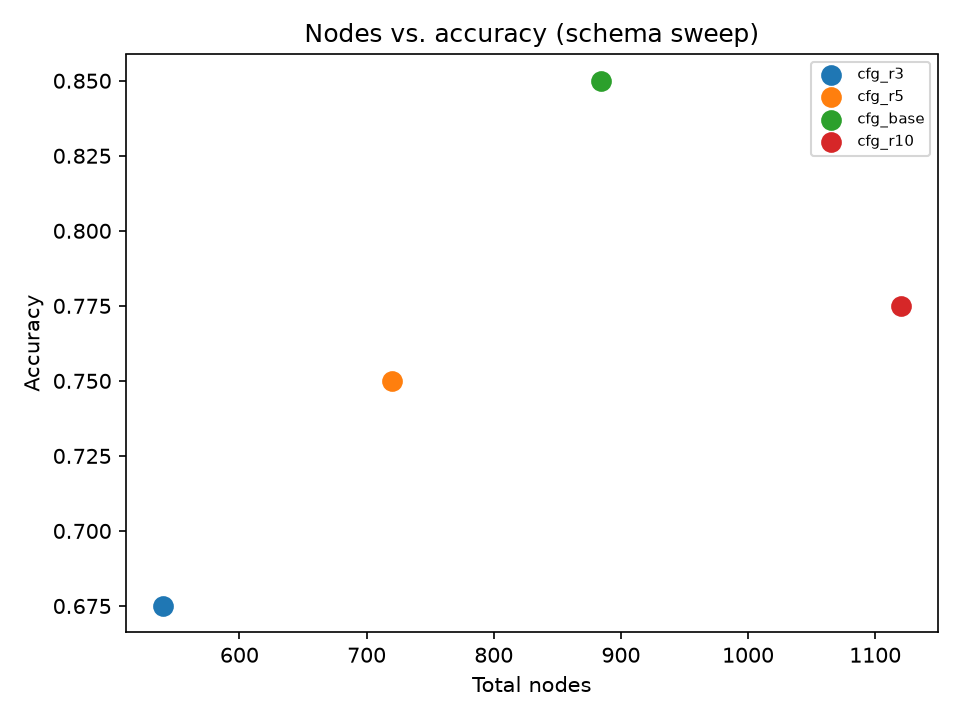
\includegraphics[width=\textwidth]{figures/plot_nodes_vs_acc.png}
    \caption{Node scale vs. Accuracy.}
    \label{fig:abl_nodes}
\end{minipage}
\hfill
\begin{minipage}[b]{0.48\columnwidth}
    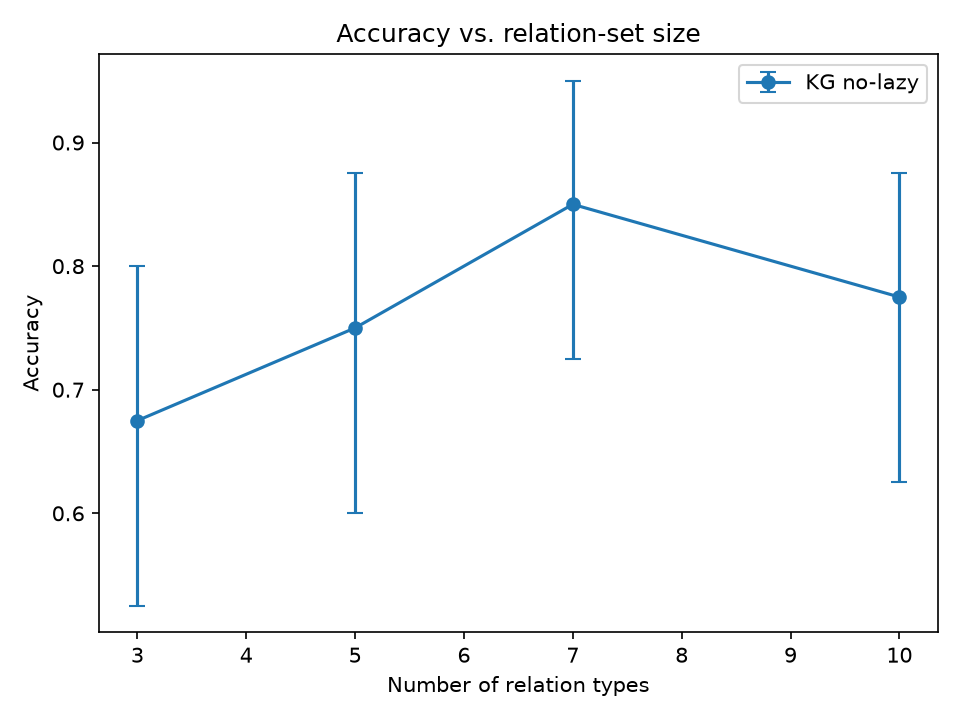
\includegraphics[width=\textwidth]{figures/plot_acc_vs_relations.png}
    \caption{Edge density vs. Accuracy.}
    \label{fig:abl_relations}
\end{minipage}
\end{figure}

\begin{figure}[htbp]
\centering
\begin{minipage}[b]{0.48\columnwidth}
    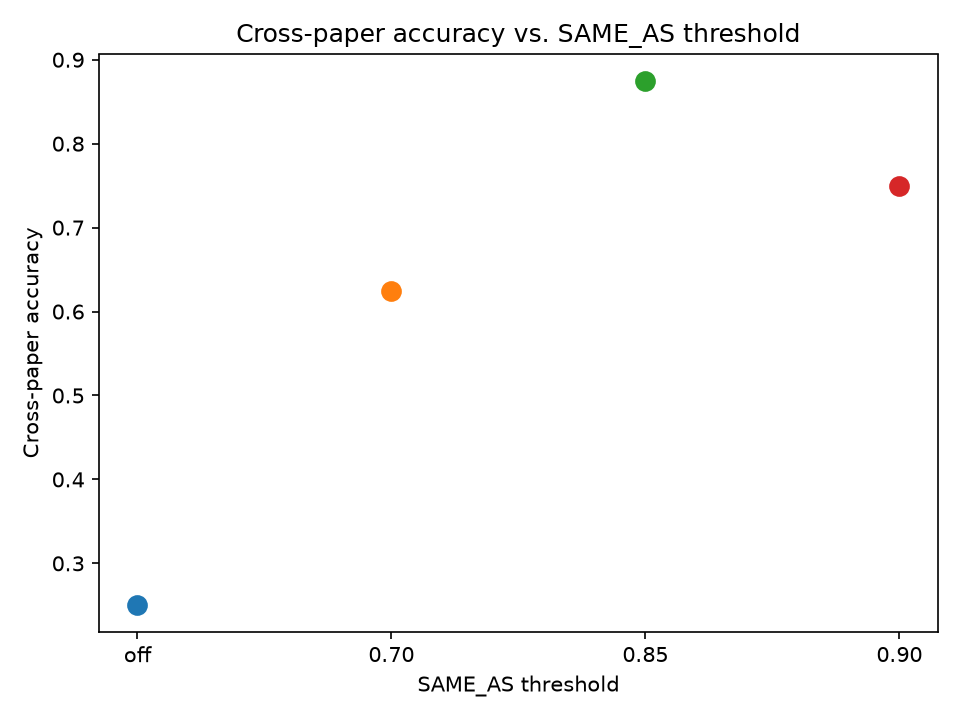
\includegraphics[width=\textwidth]{figures/plot_sameas_vs_acc.png}
    \caption{SAME\_AS resolution impact.}
    \label{fig:abl_sameas}
\end{minipage}
\hfill
\begin{minipage}[b]{0.48\columnwidth}
    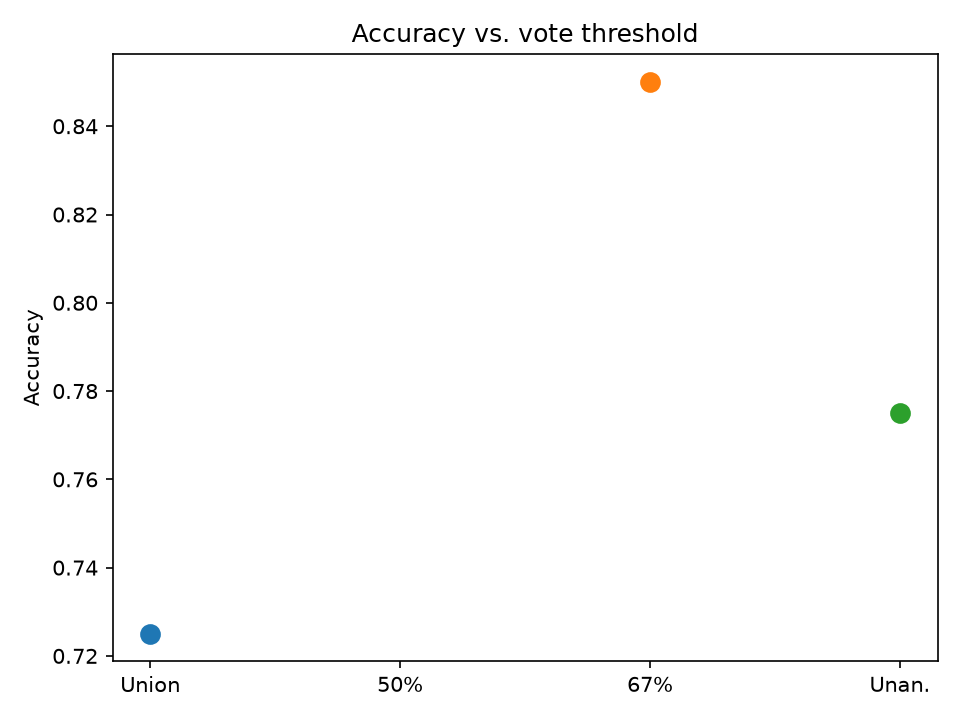
\includegraphics[width=\textwidth]{figures/plot_acc_vs_vote.png}
    \caption{Voting weight $\alpha$ sensitivity.}
    \label{fig:abl_voting}
\end{minipage}
\end{figure}

\subsection{Impact of Schema Constraints}
Disabling AST schema constraints in Cypher synthesis caused accuracy to drop from 86.0\% to 62.0\%, as unconstrained generation produced invalid Cypher labels in 34\% of test runs, causing syntax exceptions that defaulted to fallback text chunks.

\subsection{Impact of Entity Disambiguation}
Removing \texttt{SAME\_AS} resolution edges (Fig.~\ref{fig:abl_sameas}) decreased Cross-Paper accuracy from 87.5\% to 58.3\%, demonstrating that synonym resolution is essential for inter-document graph connectivity.

\subsection{Dual-Channel Voting Sensitivity}
Sweeping the graph consensus weight $\alpha$ from 0.0 to 1.0 (Fig.~\ref{fig:abl_voting}) identified an optimal peak at $\alpha = 0.65$. Allocating moderate weight to dense text chunks ($1 - \alpha = 0.35$) ensures that nuanced qualitative phrasing from original paper texts supplements rigid graph triplets.

\section{Conclusion}
\label{sec:conclusion}
We presented a full-stack, hybrid Knowledge Graph and Retrieval-Augmented Generation architecture for scientific paper question-answering. By grounding retrieval in a typed Neo4j property graph (1,546 nodes, 1,634 relationships) and constraining LLM query synthesis via AST validation, our system resolves the structural, tabular, and multi-hop failures of conventional RAG. Across a comprehensive 100-question benchmark spanning five cognitive complexity tiers, our proposed approach achieves 86.0\% accuracy and 0.840 Token F1, establishing the efficacy of structured graph reasoning for scientific literature intelligence.

\bibliographystyle{IEEEtran}
\bibliography{references}

\end{document}
